
Before we begin learning about thread-safe data structures, we have to know what they are. If this seems like a simple question – data structures that can be used by multiple threads at once – you have not given the question enough thought. I cannot overstate how important it is to ask this question every time you start designing a new data structure or an algorithm to be used in a concurrent program. If this sentence puts you on guard and gives you pause, there is a good reason for it: I have just implied that the thread-safe data structure has no single definition that suits every need and every application. This is indeed the case, and is a very important point to understand.

\subsubsubsection{7.2.1\hspace{0.2cm}The best kind of thread safety}

Let's start with something that should be obvious but is often forgotten in practice: a very general principle of designing for high performance is that doing zero work is always faster than doing some work. For the subject at hand, this general principle can be narrowed down to do you need any kind of thread-safety for this data structure? Ensuring thread safety, whatever form it takes, implies some amount of work that will need to be done by the computer. Ask yourself, do I really need it? Can I arrange the computation so that each thread has its own set of data to operate on?

A simple example is the thread-safe counter we used in the previous chapter. If you need all threads to see the current value of the counter at all times, then it was the right solution. However, let's say that all we need is to count some event that happens on multiple threads, such as searching for something in a large set of data that has been divided between the threads. A thread does not need to know the current value of the count to do the search. Of course, it would need to know the latest value of the count to increment it, but that is true only if we try to increment the single shared count on all threads, like this:

\begin{lstlisting}[style=styleCXX]
// 01a_shared_count.C
std::atomic<unsigned long> count;
…
for ( … counting loop … ) { // On each thread
	… search …
	if (… found …)
	count.fetch_add(1, std::memory_order_relaxed));
}
\end{lstlisting}

The performance of the counting itself is dismal, as can be seen in a benchmark where we do nothing but count (no search):

%\hspace*{\fill} \\ %插入空行
\begin{center}
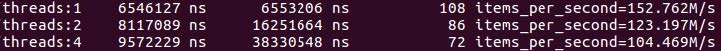
\includegraphics[width=0.9\textwidth]{content/2/chapter7/images/1.jpg}\\
Figure 7.1 – Counting on multiple threads does not scale if the count is shared
\end{center}

The scaling of the counting is actually negative: it takes longer to get to the same value of the count on two threads than on one, despite our best efforts to use a wait-free count with the minimal memory order requirements. Of course, if the search is very long compared to the counting, then the performance of the count is irrelevant (but the search code itself may present the same choice of doing some work on a global data or a per-thread copy, so consider this an instructive example).

Assuming we only care about the value of the count at the very end of the computation, a much better solution is, of course, to maintain local counts on each thread and increment the shared count only once:

\begin{lstlisting}[style=styleCXX]
// 01b_per_thread_count.C

unsigned long count;
std::mutex M; // Guards count
…
// On each thread
unsigned long local_count = 0;
for ( … counting loop … ) {
	… search …
	if (… found …) ++local_count;
}
std::lock_guard<std::mutex> L(M);
count += local_count;
\end{lstlisting}

To highlight just how unimportant the shared count increment is now, we are going to use the basic mutex; usually, a lock is a safer choice as it is easier to understand (so, harder to make bugs), although, in the case of a count, an atomic integer actually yields simpler code.

If each thread increments the local count many times before it reaches the end and has to increment the shared count, the scaling is near-perfect:

%\hspace*{\fill} \\ %插入空行
\begin{center}
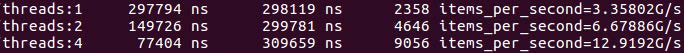
\includegraphics[width=0.9\textwidth]{content/2/chapter7/images/2.jpg}\\
Figure 7.2 – Counting on multiple threads scales perfectly with per-thread counts
\end{center}

So the best kind of thread safety is the one that is guaranteed by the fact that you don't access the data structure from multiple threads. Often, this arrangement comes at the cost of some overhead: for example, each thread maintains a container or a memory allocator whose size grows and shrinks repeatedly. You can avoid any locking whatsoever if you don't release the memory to the main allocator until the end of the program. The price will be that the unused memory on one thread is not made available to other threads, so the total memory use will be the sum of the peak uses of all threads, even if these moments of peak use occur at different times. Whether or not this is acceptable depends on the details of the problem and the implementation: it is something you have to consider for every program.

You could say that this entire section is a cop-out when it comes to thread safety. It is, from a certain point of view, but it happens so often in practice that a shared data structure is used where it is not necessary, and the performance gain can be so significant that this point needs to be made. Now it is time to move on to the real thread safety, where a data structure must be shared between threads.

\subsubsubsection{7.2.2\hspace{0.2cm}The real thread safety}

Let's assume that we really need to access a particular data structure from multiple threads at the same time. Now we have to talk about thread safety. But there is still not enough information to determine what this thread safety means. We have already discussed in the previous chapter the strong and weak thread-safety guarantees. We will see in this chapter that even that partitioning is not enough, but it puts us on the right track: instead of talking about general thread safety, we should be describing the set of guarantees provided by the data structure with regard to concurrent access.

As we have seen, the weak (but usually easy to provide) guarantee is that multiple threads can read the same data structure as long as it remains unchanged. The strongest guarantee is, obviously, that any operation can be done by any number of threads at any time, and the data structure remains in a well-defined state. This guarantee is often both expensive and unnecessary. Your program may require such a guarantee from some but not all operations supported by the data structure. There may be other simplifications, such as the number of threads accessing the data structure at once may be limited.

As a rule, you want to provide as few guarantees as necessary to make your program correct and no more: additional thread-safety features are often very expensive and create overhead even when they are not used.

With this in mind, let's start exploring concrete data structures and see what it takes to provide different levels of thread-safety guarantees.

































